\section{An exact reduction for arbitrary fixed marginal matrices}\label{sec:reduction}
The spectral formula does not directly solve the problem of a prescribed target that is misaligned with prescribed marginal matrices. An exact variational reduction does. It is valid in rectangular dimensions and for singular marginals.

Let $A$ and $B$ be density matrices on $\C^m$ and $\C^n$, and let $x=\operatorname{vec}X\in\C^m\otimes\C^n$ be a unit vector, using row-major coefficients $X_{ij}$ in $\ket{i}\otimes\ket{j}$. Then the marginals of $ww^\dagger$, for $w=\operatorname{vec}W$, are $WW^\dagger$ and $(W^\dagger W)^T$.

\begin{theorem}[Exact pure-component variational reduction]\label{thm:reduction}
Define
\[
 \mathcal W(A,B)=\{W\in\C^{m\times n}:WW^\dagger\preceq A,\ W^\dagger W\preceq B^T\}.
\]
Then
\begin{equation}\label{eq:reduction}
 \boxed{\max_{\rho_A=A,\,\rho_B=B}\bra x\rho\ket x
 =\left[\max_{W\in\mathcal W(A,B)}\Rea\tr(X^\dagger W)\right]^2
 =\left[\max_{W\in\mathcal W(A,B)}|\tr(X^\dagger W)|\right]^2.}
\end{equation}
Both maxima are attained. An optimal $W$ produces an actual optimal density matrix by a rank-one term plus a separable product residual.
\end{theorem}
\begin{proof}
If $t=\bra x\rho\ket x>0$, rank-one extraction gives $w=\rho x/\sqrt t$, $\rho\succeq ww^\dagger$ and $\langle x,w\rangle=\sqrt t$. Taking partial traces gives the two constraints on its coefficient matrix. If $t=0$, use $w=0$. This proves one inequality.

Conversely, for any feasible $W$ put $w=\operatorname{vec}W$,
\[
 A_0=A-WW^\dagger,\quad B_0=B-(W^\dagger W)^T,\quad
 \delta=\tr A_0=\tr B_0=1-\|w\|^2.
\]
When $\delta>0$,
\begin{equation}\label{eq:completion}
 \rho_W=ww^\dagger+\frac{A_0\otimes B_0}{\delta}
\end{equation}
is positive, has trace one and the required actual marginals. Its target overlap is at least $|\langle x,w\rangle|^2$. When $\delta=0$, positivity forces $A_0=B_0=0$, and $ww^\dagger$ alone is a coupling. This proves the opposite inequality. The feasible vector set is closed and bounded by $\|w\|^2\le1$, and the coupling set is compact and nonempty, so maxima exist. Finally global phase preserves the constraints on $W$ and rotates its overlap to a nonnegative real number. At a maximizing $W$, the completion must have exactly the optimal overlap; any extra positive residual contribution would contradict the already-proved equality.
\end{proof}

The positive completion formula itself has a general prior antecedent in
Remark 2.4(ii) of Skalski--Todorov--Turowska~\cite{capacity2025}.
The reduction additionally extracts a rank-one component from an arbitrary
coupling and identifies the exact target optimization, including optimizer
transfers.

\subsection{A smaller semidefinite optimization problem}
The feasible set $\mathcal W(A,B)$ is convex. By the Schur complement its constraints are equivalent to
\[
 \begin{pmatrix}A&W\\W^\dagger&\Id_n\end{pmatrix}\succeq0,
 \qquad
 \begin{pmatrix}\Id_m&W\\W^\dagger&B^T\end{pmatrix}\succeq0.
\]
Thus maximizing the real amplitude is a semidefinite program with $2mn$ real scalar variables and two positive blocks of size $m+n$. Squaring its nonnegative optimum gives the original optimum over a positive matrix of size $mn$, which has $(mn)^2$ real entries before constraints. This is an exact size reduction, not a relaxation. The numerical checks compare both formulations for independently generated, misaligned complex marginals and targets. Numerical solver tolerances are reported separately from exact proofs.

\begin{theorem}[Complementarity and a sharp optimizer-rank bound]\label{thm:rank-bound}
If $x$ has Schmidt rank $k\ge1$, some coupling maximizing its overlap has rank at most
\[
 \boxed{m+n-k.}
\]
It can be chosen as one pure positive term plus a separable residual. For a full-Schmidt target on $\C^d\otimes\C^d$, the bound becomes $d$ and is sharp even when both prescribed marginals are positive definite.
\end{theorem}
\begin{proof}
Take an optimal $W$ from Theorem~\ref{thm:reduction}. If $\delta=0$, the coupling is pure and the conclusion is immediate. Otherwise the nonnegative residual contribution in~\eqref{eq:completion} must vanish:
\[
 \bra x A_0\otimes B_0\ket x=0.
\]
The product is strictly positive on the product of its support spaces, so $x$ is orthogonal to that entire product support. Write $r=\rank A_0$ and $s=\rank B_0$. In coefficient-matrix language, $P_{A_0}X P_{B_0}^T=0$. The rank of $X$ restricted to the $s$-dimensional support of $B_0^T$ is at least $s-(n-k)$, while its image lies in a space of dimension $m-r$. Therefore
\[
 r+s\le m+n-k.
\]
In eigenbases of $A_0$ and $B_0$, couple their positive eigenvalues by a classical transportation matrix. The elementary greedy procedure matches two remaining positive masses, removes the smaller, and repeats. Each occupied cell exhausts at least one row or column, and the last exhausts both; hence it uses at most $r+s-1$ cells. The corresponding mixture of orthogonal product projectors has the same residual marginals, is supported on the same product space, and has rank at most $r+s-1$. It remains invisible to the target. Adding $ww^\dagger$ gives an optimal state of rank at most $r+s\le m+n-k$.

For $d=1$ the sharp rank is trivially one. For sharpness in the square case $d\ge2$, take $0<\eta<1/d$,
\[
 B=\Id/d,\qquad
 A=\diag\bigl(1/d+(d-1)\eta,\,1/d-\eta,\ldots,1/d-\eta\bigr),
\]
and any full-Schmidt positive diagonal target. The optimizer classification in Theorem~\ref{thm:optimizer-face} has one surplus Alice index and $d-1$ surplus Bob indices. It is unique, and its residual has rank $d-1$. The full optimizer therefore has rank exactly $d$. Both $A$ and $B$ are positive definite.
\end{proof}

The general extreme-point rank bound for fixed-marginal couplings is
$\rank\rho\le\sqrt{m^2+n^2-1}$, established by Parthasarathy~\cite{parthasarathy2003}. The target-dependent bound above can be combined with it by taking the smaller integer bound; it is not claimed to improve it for every target rank. For full-Schmidt square targets it improves the general bound to the sharp value $d$.

Klyachko's Theorem~6.4.1 already gives a coupling of prescribed marginals with rank at most the larger marginal rank, even while maximizing the spectral norm~\cite{klyachko}. Thus bare existence of a rank-$d$ coupling is established prior art. The conclusion here additionally optimizes an independently specified pure target. Applying Klyachko's theorem to $A_0,B_0$ gives the further credited existence refinement $\rank\rho\le1+\max(r,s)$; the Fourier construction below can make that residual separable. Target orthogonality of the entire residual product support preserves optimality. A further maximal-norm argument, given below, removes the extra one and establishes the stronger fixed-target bound $\max(m,n)$.

\paragraph{Subnormalized vectors are essential.}
Take $A=\diag(7/10,3/10)$, $B=\diag(3/10,7/10)$ and $x=\ket{\Phi^+}$. Every normalized pure coupling is
$\sqrt{7/10}\ket{01}+e^{i\theta}\sqrt{3/10}\ket{10}$ up to an overall phase, and has zero overlap with $x$. Nevertheless the unique optimal mixed coupling is
\[
 \rho_* =\frac3{10}(\ket{00}+\ket{11})(\bra{00}+\bra{11})
            +\frac25\ket{01}\bra{01},
 \qquad \bra x\rho_*\ket x=\frac35.
\]
Both marginals are positive and isospectral. The correct reduced optimizer has squared norm $3/5$, with its missing trace supplied by the residual. Restricting~\eqref{eq:reduction} to normalized pure couplings would therefore give a false answer.

% This standalone fragment does not overwrite the unique-core discussion.
\section{A sharp rank bound for every pure-target optimizer}
\label{sec:all-optimizer-rank}

The existence of a low-rank optimizer does not constrain the rank of other
points in an optimal face. The following theorem supplies a sharp bound for
every optimizer, including singular prescribed marginals.

For positive integers $m,n$ and $1\le k\le\min(m,n)$ define
\[
 N=m+n-k,\qquad
 R_{m,n,k}=\max\{rs:0\le r\le m,\ 0\le s\le n,\ r+s\le N,
                  \ r,s\text{ integers}\}.
\]
The elementary closed form is
\[
 R_{m,n,k}=
 \begin{cases}
 n(m-k),&m-n\ge k,\\
 m(n-k),&n-m\ge k,\\
 \lfloor(m+n-k)^2/4\rfloor,&|m-n|\le k.
 \end{cases}
\]
The formulas coincide at their shared boundaries.

\begin{theorem}[Sharp rank bound for all optimizers]
\label{thm:all-optimizer-rank}
Fix arbitrary density matrices $A,B$ on $\mathbb C^m,\mathbb C^n$ and a
unit pure target $x$ of Schmidt rank $k$. Every coupling maximizing
$\langle x,\rho x\rangle$ with these actual marginals obeys
\[
                  \boxed{\operatorname{rank}\rho\le1+R_{m,n,k}.}
\]
If the optimal target overlap is zero, the stronger bound
$\operatorname{rank}\rho\le R_{m,n,k}$ holds. No positivity assumption
on the marginal eigenvalues is needed.

For every specified unit target of Schmidt rank $k$, except the trivial
$m=n=k=1$ case, there exist positive definite marginals and an optimizer
of rank exactly $1+R_{m,n,k}$. Thus the universal bound is sharp for every
target Schmidt spectrum, not merely for one conveniently chosen target.
In square dimensions it reads
\[
 \boxed{\operatorname{rank}\rho\le
       1+\left\lfloor{(2d-k)^2\over4}\right\rfloor.}
\]
For a full-Schmidt target this is $1+\lfloor d^2/4\rfloor$.
\end{theorem}

\begin{proof}
Let $t=\langle x,\rho x\rangle$ be the optimal value. Suppose first that
$t>0$. The exact extraction
\[
 w={\rho x\over\sqrt t},\qquad R=\rho-ww^\dagger\ge0
\]
satisfies $\langle x,w\rangle=\sqrt t$ and $Rx=0$. Its residual
marginals are
\[
 A_0=A-\operatorname{Tr}_B(ww^\dagger),\qquad
 B_0=B-\operatorname{Tr}_A(ww^\dagger).
\]
They have the same nonnegative trace $\delta$. If $\delta=0$, $R=0$ and
$\rho$ is pure. Otherwise
$ww^\dagger+(A_0\otimes B_0)/\delta$ is another actual coupling.
Its overlap cannot exceed $t$, while its pure term already has overlap
$t$. Consequently
\[
                     \langle x,A_0\otimes B_0\,x\rangle=0.
\]
The product is positive definite on its support, so
$x\perp\operatorname{ran}A_0\otimes\operatorname{ran}B_0$.

Put $r=\operatorname{rank}A_0$ and $s=\operatorname{rank}B_0$.
In local bases adapted to these supports, the coefficient matrix $X$ of
$x$ has a zero $r\times s$ block. Splitting its rows and columns around
that block gives
\[
                k=\operatorname{rank}X\le(m-r)+(n-s),
                \qquad r+s\le N.
\]
Every positive matrix with residual marginals $A_0,B_0$ is supported on
their product support, so $\operatorname{rank}R\le rs$.
Since $Rx=0$ whereas $\langle x,w\rangle\ne0$, the vector $w$ is not in
$\operatorname{ran}R$. For a sum of positive matrices the range is the
sum of their ranges. Thus the ranks add exactly:
\[
        \operatorname{rank}\rho=1+\operatorname{rank}R
                             \le1+rs\le1+R_{m,n,k}.
\]

If $t=0$, the product coupling $A\otimes B$ must also have zero target
overlap. Hence $x\perp\operatorname{ran}A\otimes\operatorname{ran}B$.
Writing $r=\operatorname{rank}A$, $s=\operatorname{rank}B$, the same
zero-block argument gives $r+s\le N$. Every feasible coupling is
supported on that product space, so its rank is at most $rs\le R_{m,n,k}$.

To evaluate $R_{m,n,k}$, increasing either non-saturated variable cannot
decrease $rs$. An optimum may therefore be chosen with $r+s=N$.
Then $m-k\le r\le m$ and one maximizes the concave quadratic
$r(N-r)$ over this integer interval. The closest permitted integer to
$N/2$ gives the displayed piecewise formula.
\end{proof}

\begin{proof}[Sharpness construction]
Choose maximizing integers $r,s$ with $r+s=N$ and put
$a=m-r$, $b=n-s$. Then $a+b=k$. Outside the trivial one-dimensional
case, $r,s>0$. Write a Schmidt decomposition
\[
 x=\sum_{j=1}^{k}\sqrt{p_j}\,e_j\otimes f_j,
 \qquad p_j>0,\quad\sum_jp_j=1.
\]
Let $U$ contain the first $b$ Schmidt vectors on Alice and all of Alice's
unused Schmidt directions. Let $V$ contain the last $a$ Schmidt vectors
on Bob and all of Bob's unused Schmidt directions. Then
\[
 \dim U=b+(m-k)=r,\qquad \dim V=a+(n-k)=s,
\]
and
\[
 x\in(U\otimes V^\perp)\oplus(U^\perp\otimes V),
 \qquad x\perp U\otimes V.
\]
For any $0<q<1$ define
\[
 \rho_q=q\,xx^\dagger+{1-q\over rs}\,P_U\otimes P_V.
\]
It has rank $1+rs$. Both marginals are positive definite: the residual
is strictly positive on $U$ and $V$, while the target's nonzero Schmidt
coefficients cover their respective complements.

The local-sum operator
\[
          D=P_{U^\perp}\otimes I+I\otimes P_{V^\perp}
\]
is zero on $U\otimes V$, the identity on the two off-diagonal blocks
containing $x$, and twice the identity on
$U^\perp\otimes V^\perp$. Therefore $D\ge xx^\dagger$ and
$\operatorname{Tr}(D\rho_q)=q$. Every state with the same two marginals
has this same local-sum expectation and hence target overlap at most
$q$. The displayed state has target overlap exactly $q$, so it is an
optimizer attaining the bound. When $m=n=k=1$, the only coupling has
rank one, as claimed.
\end{proof}

\paragraph{Relation to prior rank bounds.}
Parthasarathy's general extremal-coupling bound is
$\operatorname{rank}\rho\le\sqrt{m^2+n^2-1}$
(arXiv:quant-ph/0307182). That is a statement about extreme points of the
whole coupling set. The theorem above instead concerns every point of
the exposed face selected by a pure target and tracks the target's Schmidt
rank. It complements the separate existence theorem giving an optimizer
of rank at most $\max\{\operatorname{rank}A,\operatorname{rank}B\}$. A high-rank member of the optimal face need not
be extreme. These distinctions are essential when comparing the bounds.
The precise target-dependent sharp theorem was not located in the bounded
primary-source search; historical priority has not been certified.

\paragraph{Verification scope.}
The proof is exact. The supporting rank-one extraction, positive completion,
and zero-residual-expectation steps are supplied in the finite-matrix Lean
modules. The full support/rank theorem is not claimed to be Lean formalized.
The accompanying exact-arithmetic script verifies the maximizing integer
formula, the sharp states and their local-sum dual certificates for small
rectangular dimensions and all allowed Schmidt ranks.

\subsection{What the two rank statements say in small dimensions}
For full-Schmidt targets on square systems, the existence bound and the
all-optimizer bound are both sharp, but answer different questions.
\begin{center}
\begin{tabular}{ccl}\toprule
Local dimension $d$ & Some optimizer & Every optimizer\\\midrule
2 & rank at most 2 & rank at most 2\\
3 & rank at most 3 & rank at most 3\\
4 & rank at most 4 & rank at most 5\\
5 & rank at most 5 & rank at most 7\\
6 & rank at most 6 & rank at most 10\\
8 & rank at most 8 & rank at most 17\\\bottomrule
\end{tabular}
\end{center}
For positive definite marginals, fixed full-Schmidt targets in dimensions
two and three have a unique optimizer, by the unique-core theorem below.
Dimension four permits both a nine-dimensional optimal face and rank-five
optimizers. Thus a low-rank attaining representative must not be mistaken
for a classification of all attaining states.

\section{A sharp low-rank optimizer with a separable remainder}
\label{sec:low-rank-optimizer}

The preceding rank bound controls every point of the optimal face. A stronger
existence statement holds independently of the target's Schmidt rank. It also
controls the form of an attaining ensemble.

\begin{theorem}[A low-rank pure-target optimizer]
\label{thm:low-rank-pure-target}
Let $A,B$ be arbitrary finite-dimensional density matrices, let $x$ be any
vector in their bipartite space, and put
\[
                 D=\max\{\operatorname{rank}A,\operatorname{rank}B\}.
\]
Among the states with actual marginals $A,B$, the maximum of
$\langle x,\rho x\rangle$ is attained by a state of the form
\[
 \boxed{\quad
 \rho=ww^\dagger+\sum_{j=1}^{q}p_j
                 |a_j\otimes b_j\rangle\langle a_j\otimes b_j|,
 \qquad 0\le q\le D-1,\quad p_j\ge0,
 \quad}
\]
where the local vectors $a_j,b_j$ are unit vectors. Consequently
\[
                         \boxed{\operatorname{rank}\rho\le D.}
\]
The pure core is subnormalized: $\|w\|^2+\sum_jp_j=1$.
The theorem includes singular marginals, rectangular systems, and the case
in which the optimal target overlap is zero. If the remainder is nonzero,
its product vectors can be chosen with equal weights $p_j=\delta/q$.
\end{theorem}

We first give the elementary coupling construction used in the proof.

\begin{lemma}[A short separable coupling of arbitrary marginals]
\label{lem:fourier-separable-coupling}
Suppose $E,F\ge0$ have the same positive trace $\delta$, and let
$q=\max\{\operatorname{rank}E,\operatorname{rank}F\}$. There is a
positive separable operator $R$ with marginals $E,F$ that is a sum of $q$
product projectors, and therefore has rank at most $q$. No separable
coupling with these marginals can have fewer than $q$ nonzero product
terms.
\end{lemma}

\begin{proof}
Diagonalize the marginals and pad their positive eigenvalue lists with zeros
to length $q$:
\[
 E=\sum_{i=0}^{q-1}a_i|e_i\rangle\langle e_i|,
 \qquad F=\sum_{j=0}^{q-1}b_j|f_j\rangle\langle f_j|,
 \qquad \sum_i a_i=\sum_jb_j=\delta.
\]
Terms with zero coefficients are omitted if the corresponding physical
space has dimension less than $q$. Write $\omega=e^{2\pi i/q}$ and define
\[
 u_t=\sum_i\sqrt{a_i}\,\omega^{ti}e_i,
 \qquad v_t=\sum_j\sqrt{b_j}\,\omega^{-tj}f_j,
 \qquad t=0,\ldots,q-1.
\]
Both vectors have squared norm $\delta$. Finite Fourier orthogonality gives
\[
 {1\over q}\sum_tu_tu_t^\dagger=E,
 \qquad {1\over q}\sum_tv_tv_t^\dagger=F.
\]
Hence
\[
 R={1\over q\delta}\sum_{t=0}^{q-1}
       (u_tu_t^\dagger)\otimes(v_tv_t^\dagger)
   ={\delta\over q}\sum_{t=0}^{q-1}
       \left|{u_t\over\sqrt\delta}\otimes
                    {v_t\over\sqrt\delta}\right\rangle
       \left\langle{u_t\over\sqrt\delta}\otimes
                    {v_t\over\sqrt\delta}\right|
\]
has the required marginals and is explicitly separable with $q$ terms.
Conversely, each product projector contributes rank at most one to each
marginal, so any separable ensemble requires at least
$\max\{\operatorname{rank}E,\operatorname{rank}F\}$ terms.

For comparison with a cyclic-matching construction, define
\[
 z_\ell=\sum_{i=0}^{q-1}
       \sqrt{a_i b_{i+\ell}/\delta}\;e_i\otimes f_{i+\ell},
       \qquad \ell=0,\ldots,q-1,
\]
with indices modulo $q$. The same Fourier identity gives
$R=\sum_\ell z_\ell z_\ell^\dagger$: both sides have entry
$\sqrt{a_i b_j a_k b_l}/\delta$ precisely when
$j-i=l-k\pmod q$, and entry zero otherwise. Individual $z_\ell$ may be
entangled; their sum of projectors nevertheless has the displayed
separable decomposition. Its rank is exactly $q$, because the $q$
nonzero matching vectors have disjoint supports when one eigenvalue
list has $q$ positive entries.
\end{proof}

\begin{proof}[Proof of Theorem~\ref{thm:low-rank-pure-target}]
Every feasible state is supported on
$\operatorname{ran}A\otimes\operatorname{ran}B$. Compress to these
supports and compress $x$ accordingly. Write their dimensions as $m,n$;
then $D=\max(m,n)$. The compressed target need not be a unit vector and
may vanish. The proof below allows both possibilities.

Use the coefficient-matrix convention
$w=\sum_{ij}W_{ij}|i,j\rangle$, so the pure marginal matrices are
$WW^\dagger$ and $(W^\dagger W)^T$. Set $C=B^T$ and consider
\[
 \mathcal K=\{W:\ WW^\dagger\le A,\quad W^\dagger W\le C\}.
\]
This is a nonempty compact set: it contains zero, is closed, and every
element obeys $\|W\|_F^2\le1$. It is convex, for example by the two
equivalent Schur-complement linear matrix inequalities. If $X$ is the
coefficient matrix of the compressed target, define
\[
 \tau=\max_{W\in\mathcal K}\operatorname{Re}\operatorname{Tr}(X^\dagger W).
\]
Phase invariance of $\mathcal K$ shows that this is also
$\max_{W\in\mathcal K}|\operatorname{Tr}(X^\dagger W)|$, and the exact
pure-target reduction identifies the optimal state overlap as $\tau^2$.
For completeness, the two directions of that reduction are the
rank-one extraction $w=\rho x/\sqrt{\langle x,\rho x\rangle}$ when the
denominator is nonzero, and the product-residual completion of any
feasible $w$. A zero state overlap uses $w=0$ instead. These arguments
do not require an invertible target or an invertible coupling.

Among all maximizers of the real linear objective, choose $W$ maximizing
$\|W\|_F^2$. Such a choice exists because the maximizing set is compact.
Put
\[
 E=A-WW^\dagger,\qquad F=C-W^\dagger W,
 \qquad \delta=\operatorname{Tr}E=\operatorname{Tr}F=1-\|W\|_F^2.
\]
If $\delta=0$, both residual matrices vanish, so $ww^\dagger$ is already
an optimal state of rank one. Suppose henceforth that $\delta>0$.

We claim
\[
                 \max\{\operatorname{rank}E,\operatorname{rank}F\}
                    \le D-1.                                      \tag{LR1}
\]
First assume $m\ge n$. If $E$ were positive definite, let
$V=\operatorname{ran}F$, of dimension $s\ge1$. Since
\[
                 \dim W(V^\perp)\le n-s<m,
\]
there is a nonzero vector $u\perp W(V^\perp)$. Choose any nonzero
$v\in V$ and set $Y=uv^\dagger$. Then $W^\dagger u\in V$, so all
three matrices
$W^\dagger Y$, $Y^\dagger W$, and $Y^\dagger Y$ are supported on $V$.
For sufficiently small $\varepsilon>0$, both signs satisfy
\[
 \begin{split}
 A-(W\pm\varepsilon Y)(W\pm\varepsilon Y)^\dagger
    &=E\mp\varepsilon(WY^\dagger+YW^\dagger)
                           -\varepsilon^2YY^\dagger\ge0,\\
 C-(W\pm\varepsilon Y)^\dagger(W\pm\varepsilon Y)
    &=F\mp\varepsilon(W^\dagger Y+Y^\dagger W)
                           -\varepsilon^2Y^\dagger Y\ge0.
 \end{split}
\]
The first assertion follows from strict positivity of $E$ on its full
space. The second follows from strict positivity of $F$ on $V$, since
the perturbations vanish on $V^\perp$ and have no cross blocks. Thus
both $W+\varepsilon Y$ and $W-\varepsilon Y$ lie in $\mathcal K$.
Their linear objectives average to the optimal value, so both are
themselves maximizers. But
\[
 {\|W+\varepsilon Y\|_F^2+\|W-\varepsilon Y\|_F^2\over2}
       =\|W\|_F^2+\varepsilon^2\|Y\|_F^2>\|W\|_F^2,
\]
contradicting the choice of $W$. Therefore
$\operatorname{rank}E\le m-1$. If $m>n$, also
$\operatorname{rank}F\le n\le m-1$. If $m=n$, apply the same argument
to $W^\dagger$ with the two caps exchanged to obtain
$\operatorname{rank}F\le n-1$. The case $n>m$ is symmetric. This proves
(LR1).

The product completion
\[
                ww^\dagger+{E\otimes F^T\over\delta}
\]
has marginals $A,B$. Its pure term already has target overlap $\tau^2$,
the global optimum. Consequently
\[
       \langle x,E\otimes F^T\,x\rangle=0,
       \qquad
       x\perp\operatorname{ran}E\otimes\operatorname{ran}F^T.       \tag{LR2}
\]
Here the second conclusion follows because the positive product matrix
is strictly positive on its support. The argument remains valid for
$\tau=0$: the product completion cannot have positive target overlap
when zero is the global maximum.

Apply Lemma~\ref{lem:fourier-separable-coupling} to $E,F^T$. It gives a
separable residual $R$ with these actual marginals and at most
$q=\max(\operatorname{rank}E,\operatorname{rank}F)\le D-1$ product
terms. It is supported on the space in (LR2), hence
$\langle x,Rx\rangle=0$. Therefore $\rho=ww^\dagger+R$ has the correct
actual marginals and still attains the global target optimum. Its rank
is at most $1+q\le D$, with the asserted separable decomposition.
\end{proof}

\paragraph{Sharpness in every rectangular dimension.}
The bound $D$ cannot be lowered, even for positive definite marginals.
Suppose $m\ge n$, let $A=I_m/m$, and choose a positive definite $B$ with
an eigenvalue $\beta>(m-1)/m$ and unit eigenvector $b$. For any coupling,
the positive principal block
$T=(I\otimes\langle b|)\rho(I\otimes|b\rangle)$ satisfies
$0\le T\le A$ and $\operatorname{Tr}T=\beta$. Consequently
\[
       \beta\le {\operatorname{rank}T\over m}
             \le {\operatorname{rank}\rho\over m},
       \qquad \operatorname{rank}\rho\ge m.
\]
Such $B$ exists for every $n$: for $n>1$, take the remaining eigenvalues
equal to $\varepsilon$ with
$0<\varepsilon<1/[m(n-1)]$; for $n=1$, take $B=[1]$. The case $n>m$
is symmetric. This example forces rank $D$ for every coupling, and
therefore makes the theorem sharp for every choice of target.

An explicit unique optimizer of rank $m$ is also available for a
maximal-Schmidt-rank target in every $m\ge n$ with $m>1$. Let
$0<\delta<1$, $\mu=(1-\delta)/n$, and
\[
 x={1\over\sqrt n}\sum_{i=0}^{n-1}|i,i\rangle,
 \quad w=\sqrt\mu\sum_{i=0}^{n-1}|i,i\rangle,
 \quad E={\delta\over m-1}\sum_{i=1}^{m-1}|i\rangle\langle i|.
\]
Take
\[
 A=\mu\sum_{i=0}^{n-1}|i\rangle\langle i|+E,
 \qquad B=\mu I_n+\delta|0\rangle\langle0|,
 \qquad \rho=ww^\dagger+E\otimes|0\rangle\langle0|.
\]
Both actual marginals are positive definite. Each target-diagonal
population is capped by $\mu$, so positivity and Cauchy--Schwarz give
target overlap at most $n\mu=1-\delta$, attained by this $\rho$.
For $n>1$, equality forces every target population to equal $\mu$ and
the target-diagonal principal block to be $ww^\dagger$. All remaining
nonzero populations are confined to
$\operatorname{span}\{|i,0\rangle:i\ne0\}$. Positivity therefore
writes any optimizer as
$ww^\dagger+wy^\dagger+yw^\dagger+R$ on these two blocks.
The off-diagonal Alice marginal entries with index zero force $y=0$;
the Alice marginal then forces $R=E\otimes|0\rangle\langle0|$.
Thus the displayed state is the unique optimizer and has rank $m$.
For $n=1$, the only coupling is $A\otimes B$, also of rank $m$.
For $m=n=1$, the only state has rank one.

\begin{corollary}[Fully entangled fraction and other target orbits]
For fixed actual marginals $A,B$ on $\mathbb C^d\otimes\mathbb C^d$,
the largest possible fully entangled fraction is attained by a state of
rank at most $D=\max(\operatorname{rank}A,\operatorname{rank}B)$, with
one pure core and at most $D-1$ product residual terms. The same holds
when the maximally entangled targets are replaced by any compact family
of pure targets, including a local-unitary orbit with prescribed Schmidt
coefficients.
\end{corollary}

\begin{proof}
The coupling set and the target family are compact, so choose a joint
maximizer $(\rho_*,x_*)$. Apply the theorem to the fixed target $x_*$.
The resulting low-rank state attains the joint optimal value at that
target, and therefore attains the maximum over the target family as
well. No assumption about uniqueness of the optimizing target is used.
\end{proof}

\begin{corollary}[A shorter simultaneous coherent-minimum witness]
Let $\alpha,\beta$ be probability vectors of length $d$, set
$m_i=\min(\alpha_i,\beta_i)$, $u=\alpha-m$, $v=\beta-m$, and
$\delta=\sum_i u_i=\sum_i v_i$. There is one state with actual diagonal
marginals $\operatorname{diag}\alpha,\operatorname{diag}\beta$ that
simultaneously attains
\[
 \langle x_p,\rho x_p\rangle
       =\left(\sum_i\sqrt{p_i m_i}\right)^2,
 \qquad x_p=\sum_i\sqrt{p_i}|i,i\rangle,
\]
for every probability vector $p$. If $\delta=0$, this state is pure.
Otherwise it may be chosen with rank at most
\[
           1+\max\{|\{i:u_i>0\}|,|\{i:v_i>0\}|\}\le d
\]
and with a separable residual having this same maximum number of product
terms. The displayed rank is exact when $\sum_i m_i>0$; when all
$m_i=0$, the pure core vanishes and the rank is one smaller.
\end{corollary}

\begin{proof}
Put $z=\sum_i\sqrt{m_i}|i,i\rangle$. If $\delta>0$, replace the
product residual of the coherent-minimum construction by the Fourier
coupling $R$ of $\operatorname{diag}u,\operatorname{diag}v$ from
Lemma~\ref{lem:fourier-separable-coupling}. Their positive supports are
disjoint, so $R$ is supported off the target diagonal and annihilates
every $x_p$. Thus $\rho=zz^\dagger+R$ has the displayed overlaps and
the required actual marginals. If $z\ne0$, its range is orthogonal to
the range of $R$, so the ranks add exactly. If $z=0$, all the overlaps
vanish and the same construction has rank equal to the residual rank,
which is an even stronger bound. Both residual supports are nonempty
when $\delta>0$ and are disjoint subsets of $\{1,\ldots,d\}$, so their
maximum size is at most $d-1$. If $\delta=0$, use $\rho=zz^\dagger$.
The exact target-population inequality proves optimality for each $p$;
when the spectra and weights have the required order, this also gives
a shorter attaining witness for the spectral-overlap theorem.
\end{proof}

\paragraph{Prior-art boundary and verification scope.}
The existence of some coupling with rank at most the larger marginal
rank is already Theorem~6.4.1 of A.~Klyachko,
\emph{Quantum marginal problem and representations of the symmetric
group}, arXiv:quant-ph/0409113. That theorem also discusses simultaneous
maximization of the spectral norm. The elementary Fourier ensemble
construction above is not asserted to be new. The additional statement
here is simultaneous maximization of an arbitrary prescribed pure-target
overlap, with a pure core and at most $D-1$ product residual terms.
Targeted searches of primary quantum-coupling, marginal, and quantum
transport sources did not locate this exact statement; that bounded
search does not establish publication priority. The perturbation and
rank arguments in this section are exact mathematical proofs, separate
from the Lean-verified extraction/completion reduction. No Lean
formalization of these new rank arguments is claimed.


% Fragment for inclusion in the main report. This proof is not Lean formalized.
\section{A unique coherent core for arbitrary full-rank marginals}\label{sec:unique-core}

The phase convention is essential in the following result. The reduced
optimization uses the real part of the overlap. Absolute-overlap maximizers
are determined only up to a global phase.

\begin{theorem}[Unique coherent core and the entire optimizer face]\label{thm:unique-core}
Let $A>0$ and $B>0$ be density matrices on $\mathbb C^m$ and
$\mathbb C^n$. Let $x\ne0$ have coefficient matrix $X$ of maximal rank
$\min(m,n)$. Set
\[
 M=\max\{\langle x,\rho x\rangle:
       \rho\ge0,\ \operatorname{Tr}_B\rho=A,\
       \operatorname{Tr}_A\rho=B\}.
\]
Then $M>0$, and there is a unique vector $w_*$ maximizing
$\operatorname{Re}\langle x,w\rangle$ subject to
\[
 \operatorname{Tr}_B|w\rangle\langle w|\le A,
 \qquad \operatorname{Tr}_A|w\rangle\langle w|\le B.
\]
Its overlap is $\langle x,w_*\rangle=\sqrt M$. Every density-matrix
optimizer has the same extracted vector
\[
                   \frac{\rho x}{\sqrt M}=w_*.
\]
Define $A_*=A-\operatorname{Tr}_B|w_*\rangle\langle w_*|$ and
$B_*=B-\operatorname{Tr}_A|w_*\rangle\langle w_*|$. The complete optimizer
face is precisely
\[
 \left\{|w_*\rangle\langle w_*|+R:
 R\ge0,\ \operatorname{Tr}_B R=A_*,\
 \operatorname{Tr}_A R=B_*\right\}.
\]
Every such residual is supported on
$\operatorname{ran}A_*\otimes\operatorname{ran}B_*$, a subspace
orthogonal to $x$. If $r=\operatorname{rank}A_*$ and
$s=\operatorname{rank}B_*$, then $r+s\le\max(m,n)$ whenever the residual
trace is nonzero. In the square case, every optimizer has rank at most
$1+rs\le1+\lfloor d^2/4\rfloor$, while some optimizer has rank at most $d$.
\end{theorem}

\begin{proof}
The product coupling $A\otimes B$ is positive definite. Consequently the
coupling SDP is strictly feasible, $M>0$, and its local-sum dual has an
attained optimum:
\[
 D=H\otimes I+I\otimes K\ \ge\ |x\rangle\langle x|,
 \qquad \operatorname{Tr}(HA)+\operatorname{Tr}(KB)=M.
\]
This is the standard quantum-coupling dual; see Cole et al., Theorem~3.2~\cite{cole2023}. Since $D\ge0$,
$\lambda_{\min}(H)+\lambda_{\min}(K)\ge0$. Replacing
$H$ by $H-\lambda_{\min}(H)I$ and $K$ by
$K+\lambda_{\min}(H)I$ leaves both $D$ and the dual objective unchanged
and makes $H,K\ge0$.

Put $U=\ker H$, $V=\ker K$, and $T=U\otimes V=\ker D$.
The inequality $D\ge|x\rangle\langle x|$ implies $x\perp T$. On
$T^\perp$, $D$ is positive definite. Let $v=D^+x$, where $D^+$ is the
Moore--Penrose inverse, and let $\gamma=\langle x,D^+x\rangle$.
Congruence with $D^{+1/2}$ gives $0<\gamma\le1$. If $\gamma<1$, then
the slack $Z=D-|x\rangle\langle x|$ has kernel exactly $T$.
Complementary slackness would then force every optimal $\rho$ to be
supported on $T$, giving $\langle x,\rho x\rangle=0$, contrary to $M>0$.
Thus $\gamma=1$ and
\[
      \ker Z=\mathbb Cv\oplus T,\qquad
      \langle x,v\rangle=1,\qquad v\perp T.
\]
These assertions also follow directly from
$Zq=0\iff Dq=x\langle x,q\rangle$ after splitting off $\ker D$.

Set $z=\sqrt M\,v$. Any optimal $\rho$ is supported on
$\mathbb Cz\oplus T$ and has the unique block form
\[
 \rho=|z\rangle\langle z|+|z\rangle\langle y|
            +|y\rangle\langle z|+R,
 \quad y\in T,\quad R\text{ supported on }T,\quad R\ge|y\rangle\langle y|.
\]
Indeed the scalar coefficient of $|z\rangle\langle z|$ is fixed to one
by $\langle x,z\rangle=\sqrt M$ and the optimal objective $M$; positivity
gives the stated Schur-complement condition. Also
$\rho x/\sqrt M=z+y$.

It remains to prove that $y$ is independent of the optimizer. Choose
orthonormal local bases diagonalizing $H,K$. In these bases write $Z_0$,
$Y$ for the coefficient matrices of $z,y$. Then $Y$ is supported on the
$U\times V$ block and $(Z_0)_{U,V}=0$, while
\[
                   HZ_0+Z_0K^{\mathsf T}=\sqrt M\,X.
\]
Suppose first $m\ge n$, so $X$ is injective. On the columns indexed by
$V$ the preceding identity becomes
\[
   (Z_0)_{U^\perp,V}
      =\sqrt M\,(H|_{U^\perp})^{-1}X_{U^\perp,V}.
\]
Because $X_{U,V}=0$ and $X$ is injective, this matrix has full column
rank. For two optimizers subtract their $A$-marginal equations and take
the $U^\perp\times U$ block. The pure core cancels, the residual terms
have support in $U\times U$, and one obtains
\[
              (Z_0)_{U^\perp,V}(Y_1-Y_2)^*=0.
\]
Full column rank therefore gives $Y_1=Y_2$. If $m\le n$, apply the same
argument to the other marginal and $X^*$, which is injective. Empty
$U$ or $V$ cause no exception: then $T=0$ and $y=0$ immediately.

Write the common vector $z+y$ as $w_*$. Completing the square shows
\[
 \rho=|w_*\rangle\langle w_*|+(R-|y\rangle\langle y|).
\]
Thus every optimizer has the asserted positive residual, supported on
$T$ and with marginals $A_*,B_*$. Conversely, $\operatorname{ran}A_*
\subseteq U$ and $\operatorname{ran}B_*\subseteq V$. Every positive
coupling of these marginals is supported on
$\operatorname{ran}A_*\otimes\operatorname{ran}B_*\subseteq T$, so it is
orthogonal to $x$ and yields objective $M$ after adding the fixed pure
core. This proves the face description.

Any reduced real-overlap optimizer $w$ has
$\langle x,w\rangle=\sqrt M$. A positive completion
$\rho\ge|w\rangle\langle w|$ is optimal by the exact reduction. Its
residual has zero expectation in $x$, hence annihilates $x$, and
$\rho x/\sqrt M=w$. Therefore $w=w_*$, proving uniqueness, including
the real-overlap phase convention.

Finally $x\perp\operatorname{ran}A_*\otimes\operatorname{ran}B_*$
means that its coefficient matrix contains a zero $r\times s$ block.
Hence $\operatorname{rank}X\le(m-r)+(n-s)$ and
$r+s\le m+n-\operatorname{rank}X=\max(m,n)$. Every residual has rank
at most $rs$. A classical transport coupling of the eigenvalue lists of
$A_*,B_*$ can be chosen with at most $r+s-1$ nonzero cells and gives a
residual of that rank. The stated rank bounds follow, with the zero
residual case handled by the pure state itself.
\end{proof}

\begin{corollary}[The first dimension with nonunique fixed-target optimizers]
For positive definite marginals on $\mathbb C^d\otimes\mathbb C^d$ and a full-Schmidt-rank fixed pure target, the optimizing density matrix is unique whenever $d\le3$.
If the residual trace is nonzero, the full optimizer face has real affine dimension
$(r^2-1)(s^2-1)$, where $r,s$ are its residual marginal ranks. It is unique exactly when $\min(r,s)=1$. The zero-residual case is also unique.
Dimension four is the first square dimension permitting nonuniqueness under these hypotheses; the $25/36$ family below realizes a nine-dimensional face.
\end{corollary}
\begin{proof}
The residual product coupling is positive definite on the product of the residual supports, so the fixed-marginal affine space has its full dimension $r^2s^2-r^2-s^2+1$. This is positive precisely when $r,s\ge2$. If $d\le3$, the inequality $r+s\le d$ excludes that case. Addition of the fixed pure core is injective and affine. This is a fixed-target statement; it does not assert uniqueness when the maximally entangled target itself is also varied in the definition of FEF.
\end{proof}

\begin{corollary}[Support-compressed unique core]
Let $A,B$ be arbitrary density matrices, and compress the target to
$x'=(P_A\otimes P_B)x$, where $P_A,P_B$ project onto their supports.
If the coefficient matrix of $x'$ has rank
$\min(\operatorname{rank}A,\operatorname{rank}B)$, the unique-core and
complete residual-face conclusions hold on those support spaces. Their
dimension and rank bounds use $\operatorname{rank}A$ and
$\operatorname{rank}B$ in place of the ambient local dimensions.
\end{corollary}
\begin{proof}
Every feasible positive coupling, and every feasible reduced vector, is
supported on $\operatorname{ran}A\otimes\operatorname{ran}B$. Indeed,
a zero marginal expectation on a local vector forces every corresponding
joint diagonal expectation to vanish; positivity then annihilates that
entire local-kernel tensor factor. Compressing therefore changes neither
optimization problem. On that product space the two marginals are
positive definite, and the unique-core theorem applies. Its proof permits
an arbitrary nonzero target, so no normalization of $x'$ is needed.
\end{proof}


\paragraph{Why strict positivity matters.}
Take $A=\operatorname{diag}(1/2,1/2,0)$,
$B=\operatorname{diag}(1/2,0,1/2)$ and
$x=(|00\rangle+|11\rangle+|22\rangle)/\sqrt3$.
The exact optimum is $M=1/6$. Both
\[
 w_0=|00\rangle/\sqrt2,
 \qquad w_1=(|00\rangle+|12\rangle)/\sqrt2
\]
are admissible and have real overlap $1/\sqrt6$. Thus a full-Schmidt-rank
target alone does not force uniqueness. The missing positive-definiteness
assumption cannot be silently replaced by nonnegative marginals.

\paragraph{Why maximal Schmidt rank matters.}
Take $A=B=I_2/2$ and the product target $x=|00\rangle$. The optimum is
$M=1/2$, and both $w_0=|00\rangle/\sqrt2$ and
$w_1=(|00\rangle+|11\rangle)/\sqrt2$ are reduced real-overlap
optimizers. Thus positive definite marginals alone do not give a unique
coherent core.

\subsection{An exact noncommuting example with a nonzero cross component}
The proof fixes the cross vector $y$; it does not generally make $y$ zero.
An explicit example is
\[
 x=\frac13(2,0,1,2)^T,\qquad
 A=\frac1{100}\begin{pmatrix}83&8\\8&17\end{pmatrix},\qquad
 B=\frac1{100}\begin{pmatrix}17&8\\8&83\end{pmatrix}.
\]
Both marginals are positive definite. The unique optimizer is
\[
 \rho_* =\frac1{100}
 \begin{pmatrix}
 16&4&4&16\\4&67&1&4\\4&1&1&4\\16&4&4&16
 \end{pmatrix}
 =w_*w_*^\dagger+\frac{33}{50}|01\rangle\langle01|,
 \quad w_*=\frac1{10}(4,1,1,4)^T.
\]
Its overlap is $289/900$. An exact dual certificate is
\[
 D=\frac{17}{18}\diag(1,0,2,1),\qquad
 D-xx^\dagger=\frac{17aa^\dagger+bb^\dagger}{36}\succeq0,
\]
where $a=(1,0,0,-1)^T$ and $b=(1,0,-8,1)^T$. The local dual objective is also $289/900$, proving optimality without a numerical solver.
In the proof's decomposition, $z=(4,0,1,4)^T/10$ and $y=|01\rangle/10\ne0$.
All entries, principal-minor positivity checks, partial traces, the dual decomposition, and the uniqueness equations on the dual kernel are verified with exact rational arithmetic in the accompanying script.

\paragraph{Status and prior art.}
The local-sum dual, complementary slackness, and positive-marginal dual
attainment are standard and explicitly established in
arXiv:2105.06922v2, Theorem~3.2. The unique-core and complete residual-face
conclusions above are derived here. A bounded primary-source
search did not locate this precise theorem; this is a novelty candidate,
not a certified priority claim. The proof above is exact mathematics, not
an asserted Lean result. The \texttt{FixedMarginalReduction} section of \texttt{AllProofs.lean} establishes the actual finite-matrix
reduction and optimizer transfer on which it relies.


\section{Fixed marginal matrices: the whole optimizer set}\label{sec:face}
The spectral theorem has a second, basis-sensitive version. It also exposes much more of the equality geometry than a single attaining example. This section fixes the actual marginal matrices and the target vector, not only their spectra. No ordering of the diagonal entries is required.

Let $a,b,p\in\R^d$ be probability vectors, with $p_i>0$ for every $i$. Put
\[
 A=\diag(a),\quad B=\diag(b),\quad
 x=\sum_i\sqrt{p_i}\ket{ii},\quad
 m_i=\min(a_i,b_i),\quad u=a-m,\quad v=b-m,
\]
\[
 z=\sum_i\sqrt{m_i}\ket{ii},\qquad
 L=\sum_i m_i,\qquad \delta=1-L,\qquad
 S=\sum_i\sqrt{p_i m_i}.
\]
Define $I_+=\{i:a_i>b_i\}$ and $I_-=\{i:b_i>a_i\}$, and the orthogonal subspaces
\[
 E_+=\operatorname{span}\{\ket i:i\in I_+\},\quad
 E_-=\operatorname{span}\{\ket i:i\in I_-\},\quad
 \mathcal T=E_+\otimes E_-.
\]
The entries of $u$ and $v$ have disjoint supports. Unless $a=b$, both $I_+$ and $I_-$ are nonempty.

\begin{theorem}[Exact fixed-matrix overlap optimum]\label{thm:fixed-matrix}
For all bipartite density matrices with $\rho_A=A$ and $\rho_B=B$,
\[
 \boxed{\max_\rho\bra x\rho\ket x=S^2.}
\]
This holds also when $a$ or $b$ has zero entries. The statement fixes the diagonal marginal matrices in the target's Schmidt bases; it is not a formula for arbitrary misaligned fixed matrices and a prescribed target.
\end{theorem}
\begin{proof}
Write $d_i=\rho_{ii,ii}$. Marginal positivity gives $0\le d_i\le a_i,b_i$, hence $d_i\le m_i$. Positive semidefiniteness gives $|\rho_{ii,jj}|\le\sqrt{d_i d_j}$. Therefore
\[
 \bra x\rho\ket x
 \le\sum_{ij}\sqrt{p_i p_j}\,|\rho_{ii,jj}|
 \le\left(\sum_i\sqrt{p_i d_i}\right)^2
 \le S^2.
\]
For $\delta>0$, the state
\[
 zz^\dagger+\frac1\delta\diag(u)\otimes\diag(v)
\]
has the required marginals and overlap $S^2$, since $u_i v_i=0$. For $\delta=0$, $a=b=m$ and $zz^\dagger$ attains the bound. This is an actual matrix optimization, with no singular-value existence assumption.
\end{proof}

\begin{theorem}[Complete optimizer face for positive marginal entries]\label{thm:optimizer-face}
Suppose every $m_i>0$. The complete set of optimizers in Theorem~\ref{thm:fixed-matrix} consists precisely of
\begin{equation}\label{eq:optimizer-face}
 \boxed{\rho=zz^\dagger+R,\quad R\succeq0,\quad
 \operatorname{ran}R\subseteq\mathcal T,\quad
 R_A=\diag(u),\quad R_B=\diag(v).}
\end{equation}
Thus the freedom in the optimizer is exactly a smaller quantum coupling problem on $E_+\otimes E_-$.
\end{theorem}
\begin{proof}
Equality throughout the preceding proof first forces $d_i=m_i$: all $\sqrt{p_i}$ are strictly positive and the scalar square root is strictly increasing. Equality in the entrywise sum forces the whole diagonal-coordinate block to be $\rho_{ii,jj}=\sqrt{m_i m_j}$. Every off-diagonal basis vector $\ket{ij}$, $i\ne j$, outside $\mathcal T$ has zero population. Indeed, either $u_i=0$, which exhausts row $i$'s marginal population at $\ket{ii}$, or $v_j=0$, which exhausts column $j$'s population at $\ket{jj}$. A zero diagonal entry of a positive matrix forces its entire row and column to vanish.

Relative to the diagonal-coordinate space and $\mathcal T$, a positive matrix whose first block is $zz^\dagger$ must have the form
\[
 \rho=zz^\dagger+zy^\dagger+yz^\dagger+R,
 \qquad y\in\mathcal T,\qquad R\succeq yy^\dagger.
\]
This follows either from the rank-one Schur complement or by testing the kernel of $zz^\dagger$. For $i\in I_+$ and $j\in I_-$, the off-diagonal entry $(j,i)$ of $\rho_A$ receives from the cross block the unique contribution $\sqrt{m_j}\,\overline{y_{ij}}$. The residual $R_A$ is supported on $E_+$, so it cannot cancel this entry. Likewise the corresponding entry of $\rho_B$ is proportional to $\sqrt{m_i}\,y_{ij}$. Both prescribed marginals are diagonal, and $m_i,m_j>0$, so $y_{ij}=0$. Hence $y=0$ and the remaining marginal equations are exactly those in~\eqref{eq:optimizer-face}. Conversely every state in~\eqref{eq:optimizer-face} has the prescribed marginals and the same overlap, since $x\perp\mathcal T$.
\end{proof}

\begin{corollary}[Uniqueness, dimension and rank]\label{cor:face-dimension}
Let $r=|I_+|$ and $s=|I_-|$. Under the hypotheses of Theorem~\ref{thm:optimizer-face}:
\begin{enumerate}
\item If $a=b$, the optimizer is the pure state $zz^\dagger$.
\item If $a\ne b$, the optimizer is unique if and only if $\min(r,s)=1$.
\item If $r,s\ge2$, its face has real affine dimension
\[
 (r^2-1)(s^2-1).
\]
\item Every optimizer satisfies $\rank\rho=1+\rank R\le1+rs$. The upper rank is attained by $R=\diag(u)\otimes\diag(v)/\delta$.
\end{enumerate}
In particular no optimizer of this positive-marginal problem is full rank for $d\ge2$.
\end{corollary}
\begin{proof}
If either residual local space has dimension one, its fixed marginal determines $R$ uniquely. Otherwise the Hermitian operators on an $r s$-dimensional space have real dimension $r^2s^2$. Prescribing both marginals imposes $r^2+s^2-1$ independent real linear constraints, with the trace counted once. Independence follows by allowing arbitrary traceless perturbations of either marginal and one common trace perturbation. The product residual is positive definite on $\mathcal T$, so the feasible set has the full affine dimension claimed. Its dimension is positive exactly when $r,s\ge2$. Finally $z\perp\mathcal T$, so the ranks add. Since $r+s\le d$, $1+rs\le1+\lfloor d^2/4\rfloor<d^2$ for $d\ge2$.
\end{proof}

\subsection{The boundary: extra coherences are real}
For completeness the zero-entry case can also be classified exactly. Set
\[
 Z_+=\{i\in I_+:m_i=0\},\qquad
 Z_-=\{i\in I_-:m_i=0\},\qquad
 \mathcal T_0=\operatorname{span}\{\ket{ij}:i\in Z_+,j\in Z_-\}.
\]
\begin{theorem}[Complete boundary parametrization]\label{thm:boundary-face}
If $L>0$, all optimizers in Theorem~\ref{thm:fixed-matrix} are precisely
\begin{equation}\label{eq:boundary-face}
 \rho=zz^\dagger+zy^\dagger+yz^\dagger+R,
 \quad y\in\mathcal T_0,\quad R-yy^\dagger\succeq0,
\end{equation}
where $R$ is supported on $\mathcal T$ and has marginals $\diag(u),\diag(v)$. If $L=0$, the optimum is zero and every coupling with the prescribed marginals is optimal.
\end{theorem}
\begin{proof}
The same equality and positivity argument gives the rank-one first block, the allowed support, and $R\succeq yy^\dagger$. The off-diagonal marginal equations now give only $\sqrt{m_i}y_{ij}=\sqrt{m_j}y_{ij}=0$. These are exactly $y\in\mathcal T_0$. Conversely such cross terms have both partial traces zero, and are orthogonal to $x$ on their residual side, so they preserve the marginals, trace and optimal overlap. The Schur-complement condition is exactly positivity. When $L=0$, no coordinate $\ket{ii}$ can have positive population, hence every admissible positive state annihilates the target.
\end{proof}

For example, $a=(1/2,1/2,0)$ and $b=(1/2,0,1/2)$ have $m=(1/2,0,0)$. For every full-Schmidt diagonal target,
\[
 \rho=\tfrac12(\ket{00}+\ket{12})(\bra{00}+\bra{12})
\]
is an optimizer. Its cross terms are nonzero. Dropping the positivity assumption on $m$ in~\eqref{eq:optimizer-face} would therefore be false.

\section{An exact dual certificate and a singular nonattainment theorem}\label{sec:dual}
The local-sum dual and its positive-marginal attainment are established quantum-transport tools~\cite{cole2023}. That paper also gives a singular two-qubit example of nonattainment and the zero-row obstruction used below. The additions here are an explicit certificate for the whole diagonal pure-target problem, its kernel and support estimate, and a general zero-entry criterion. Assume $m_i>0$. Put
\[
 \ell_i=S\sqrt{p_i/m_i},\qquad
 h_i=\begin{cases}\ell_i&a_i<b_i,\\0&a_i>b_i,\\\ell_i/2&a_i=b_i,\end{cases}
 \qquad k_i=\ell_i-h_i.
\]
Let $H=\diag(h)$, $K=\diag(k)$, and
\[
 Z=H\otimes\Id+\Id\otimes K-xx^\dagger.
\]
\begin{theorem}[Dual certificate and robust support]\label{thm:dual}
The operator $Z$ is positive semidefinite,
\[
 \tr(HA)+\tr(KB)=S^2,
 \qquad \ker Z=\operatorname{span}\{z\}\oplus\mathcal T.
\]
If $P$ projects onto this kernel and $\ell_{\min}=\min_i\ell_i$, then
\[
 Z\succeq\frac{\ell_{\min}}2(\Id-P).
\]
Consequently every admissible $\rho$ with overlap deficit $\epsilon=S^2-\bra x\rho\ket x$ satisfies
\begin{equation}\label{eq:support-stability}
 \boxed{\tr((\Id-P)\rho)\le\frac{2\epsilon}{\ell_{\min}}.}
\end{equation}
If the right side is less than one, there is a normalized state $\widehat\rho$ supported on $\ker Z$ with
\[
 \|\rho-\widehat\rho\|_1\le2\sqrt{2\epsilon/\ell_{\min}}.
\]
This last state is not asserted to have exactly the original marginals. The conclusion is a quantitative support theorem, not an unstated distance bound to the entire optimizer face.
\end{theorem}
\begin{proof}
On diagonal coordinates, $Z=D-xx^\dagger$ with $D=\diag(\ell)$ and
\[
 x^\dagger D^{-1}x=\sum_i p_i/\ell_i=1.
\]
Thus $D^{-1/2}ZD^{-1/2}$ is an orthogonal projection. Its kernel corresponds to $D^{-1}x=z/S$, and its nonzero eigenvalues are at least $\ell_{\min}$: the nonzero spectra of $D^{1/2}(\Id-aa^\dagger)D^{1/2}$ and $(\Id-aa^\dagger)D(\Id-aa^\dagger)$ agree, where $a=D^{-1/2}x$ is unit. On an off-diagonal coordinate $\ket{ij}$ the coefficient is $h_i+k_j$. It is zero exactly for $i\in I_+,j\in I_-$, and otherwise at least $\ell_{\min}/2$. This proves the operator and kernel assertions. The dual objective is $\sum_i m_i\ell_i=S^2$, so $\epsilon=\tr(Z\rho)$ and~\eqref{eq:support-stability} follows. Finally use $\widehat\rho=P\rho P/\tr(P\rho)$ and a purification projected onto $P$: its overlap with the original purification is $\sqrt{\tr(P\rho)}$. The pure-state trace-distance formula and contractivity under partial trace give the displayed bound.
\end{proof}

\begin{theorem}[A sharp boundary failure of dual attainment]\label{thm:dual-noattain}
Suppose $p_i>0$ for every $i$, $L>0$, and $m_j=0$ for at least one $j$. The primal optimum $S^2$ is attained, but no finite Hermitian matrices $H,K$ attain the matching dual problem
\[
 \inf\{\tr(HA)+\tr(KB):H\otimes\Id+\Id\otimes K\succeq xx^\dagger\}.
\]
The infimum still equals $S^2$.
\end{theorem}
\begin{proof}
For $\eta>0$ define $m_i^{(\eta)}=m_i+\eta$, $S_\eta=\sum_i\sqrt{p_i(m_i+\eta)}$ and $\ell_i^{(\eta)}=S_\eta\sqrt{p_i/(m_i+\eta)}$. Split each coefficient between $H$ and $K$ according to the smaller actual marginal entry, as above. The same diagonal weighted-Cauchy argument gives a feasible dual pair, with objective
\[
 C_\eta=\sum_i m_i\ell_i^{(\eta)}\longrightarrow S^2.
\]
Weak duality and the explicit primal optimizer prove equality of the infimum. If finite multipliers attained it, their positive slack $Z$ would obey $\tr(Z\rho_*)=0$ for the explicit primal state $\rho_*=zz^\dagger+R_*$ with $R_*\succeq0$. Hence $Zz=0$. But at the coordinate $(j,j)$ with $m_j=0$, any local-sum operator obeys
\[
 [(H\otimes\Id+\Id\otimes K)z]_{jj}=0,
\]
whereas $(xx^\dagger z)_{jj}=\sqrt{p_j}S>0$. This contradiction proves nonattainment. The assumption $L>0$ is essential; when $L=0$, an optimal dual of objective zero can be constructed by assigning positive diagonal coefficients only to zero-cost marginal entries.
\end{proof}

\begin{figure}[htbp]\centering
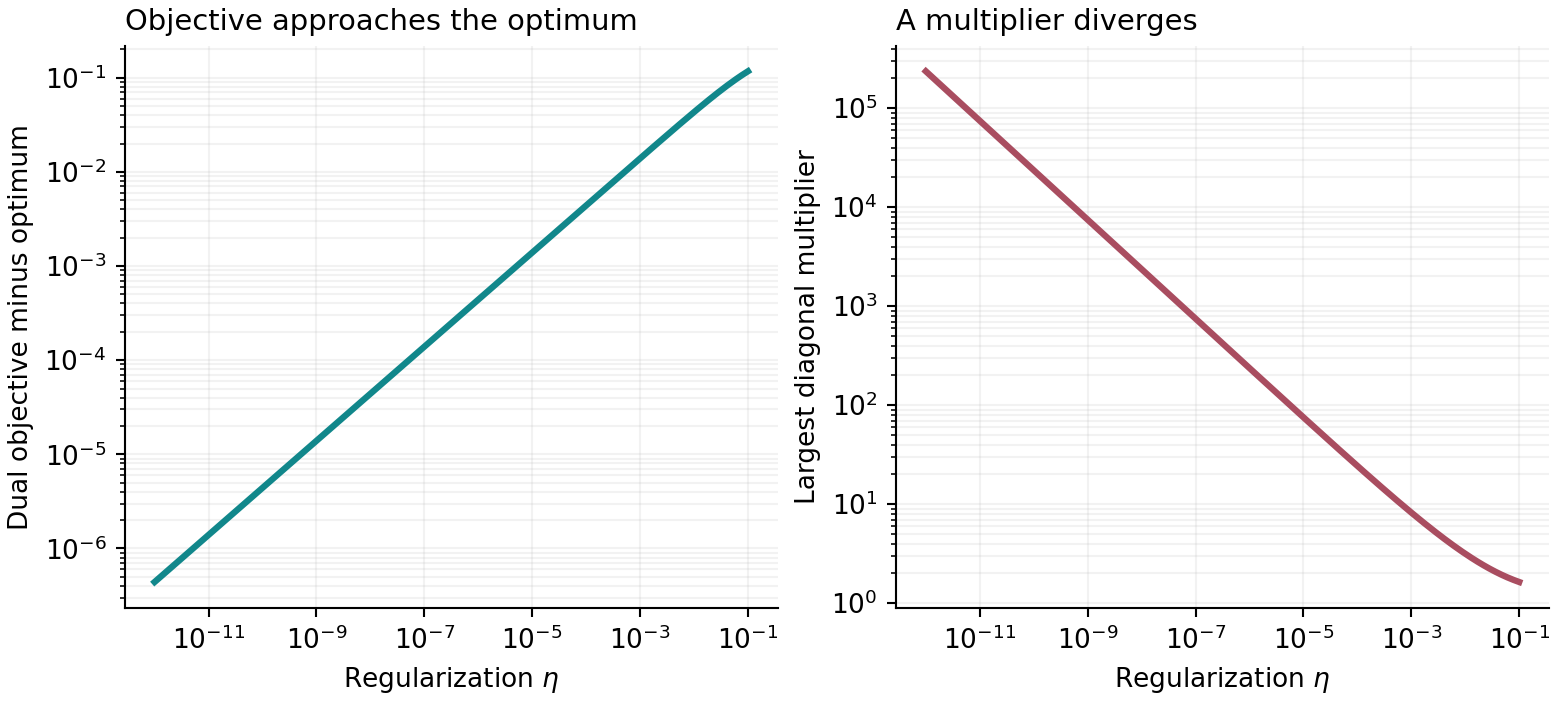
\includegraphics[width=\textwidth]{singular_dual_limit.png}
\caption{The explicit feasible dual sequence for $a=(0.3,0.2,0.5,0)$, $b=(0.3,0.2,0,0.5)$ and $p=(0.1,0.2,0.3,0.4)$. Its objective converges to the attained primal optimum while a multiplier diverges. Curves evaluate the exact formula; they are not solver output.}
\end{figure}

\section{Universality of higher-dimensional equality sets}\label{sec:universality}
The optimizer face is large enough to contain an arbitrary smaller bipartite fixed-marginal problem. This explains why a qubit-like unique normal form should not be expected in higher dimension.

\begin{theorem}[Embedding arbitrary residual quantum correlations]\label{thm:universality}
Let $\omega$ be any density matrix on $\C^r\otimes\C^s$ with specified marginals. There exist positive probability vectors $a,b$ in dimension $d=r+s$, with both lists decreasing, and an affine embedding of the whole fixed-marginal state space of $\omega$ into the optimizers of the marginal-spectrum FEF bound. Each embedded state has the form
\[
 \rho_\omega=zz^\dagger+\delta V\omega V^\dagger,\qquad \delta>0,
\]
and satisfies
\[
 f_d(\rho_\omega)=\frac1d\left(\sum_i\sqrt{m_i}\right)^2,
 \qquad \rank\rho_\omega=1+\rank\omega.
\]
The local product projection onto the residual subspaces extracts $V\omega V^\dagger$ with probability exactly $\delta$.
\end{theorem}
\begin{proof}
Diagonalize the two prescribed marginals of $\omega$, with eigenvalue vectors $a',b'$. Choose a strictly decreasing positive probability vector $\lambda$ of length $d$. Allocate disjoint index sets of sizes $r,s$ to the two residual spaces, and embed $a',b'$ on these respective sets as $\widetilde a,\widetilde b$. Choose $0<\delta<1$ sufficiently small that
\[
 \delta\max(\|\widetilde a\|_\infty,\|\widetilde b\|_\infty)
 <(1-\delta)\min_{i<d-1}(\lambda_i-\lambda_{i+1}).
\]
Set $m=(1-\delta)\lambda$, $a=m+\delta\widetilde a$ and $b=m+\delta\widetilde b$. They remain strictly decreasing positive probability vectors, and their componentwise minimum is $m$. The isometry $V$ embeds $\omega$ in the product of the disjoint residual spaces. The displayed state has marginals $\diag(a),\diag(b)$ and its Bell overlap is $(\sum\sqrt m)^2/d$. The universal spectral theorem proves that no other maximally entangled target does better. Orthogonality of the coherent and residual supports gives the rank identity and the local-projection statement. All choices depend only on the prescribed marginal pair, so the embedding is affine on the entire corresponding coupling space.
\end{proof}

\subsection{An exact four-dimensional family with different residual entanglement}
Take
\[
 m=\frac1{36}(16,9,4,1),\qquad
 a=\frac1{36}(19,9,7,1),\qquad
 b=\frac1{36}(16,12,4,4),\qquad\delta=\frac16.
\]
Here $I_+=\{0,2\}$, $I_-=\{1,3\}$, and
\[
 z=\frac16(4\ket{00}+3\ket{11}+2\ket{22}+\ket{33}).
\]
Let $\omega$ be any two-qubit state with both marginals $\Id_2/2$, embedded by $V\ket{i,j}=\ket{2i,2j+1}$. Then
\[
 \rho_\omega=zz^\dagger+\frac16V\omega V^\dagger,
 \qquad \boxed{f_4(\rho_\omega)=\frac{25}{36}.}
\]
For $\omega=\ket{\Phi^+}\bra{\Phi^+}$ the full state has rank two, and local projection onto even Alice and odd Bob levels yields a Bell pair with probability $1/6$. For $\omega=\Id_4/4$ the full state has rank five and the same projection yields a separable state. Both have exactly the same actual marginals and fully entangled fraction. The optimizer face has affine dimension nine. The coherent-plus-product sharpness witness is therefore only one point in a much larger equality set.

\section{Success probability versus conditional entangled fraction}\label{sec:success}
Local filtering is operational only after specifying its success probability. Here the input is a canonical two-qubit state $\sigma$ with $\sigma_B=\Id/2$ and centre length $c$. A single successful Bob Kraus operator $K$ satisfies $K^\dagger K\preceq\Id$; the successful state is normalized by its probability $q_K$.

\begin{theorem}[Sharp required-success frontier]\label{thm:success}
Let $0\le c\le1$ and $0<q\le1$. Over all such canonical inputs and filters with success probability at least $q$, the maximal conditional FEF is
\begin{equation}\label{eq:success-frontier}
 \boxed{
 G(c,q)=\begin{cases}
 1-c/2,&0<q\le1-c/2,\\[2mm]
 \displaystyle\frac{[1+\sqrt{(1-c)(2q-1)}]^2}{4q},&1-c/2\le q\le1.
 \end{cases}}
\end{equation}
Every value is attained. The two expressions agree at the transition. At $q=1$, the frontier is the canonical bound; allowing success $q=1-c/2$ reaches Milne's larger centre-only bound.
\end{theorem}
\begin{proof}
The input Bob marginal is uniform, so $q_K=\tr(K^\dagger K)/2$. If the normalized output Bob length is $b$, the two eigenvalues of $K^\dagger K$ are $q_K(1+b)$ and $q_K(1-b)$. Physical admissibility therefore implies
\[
 q_K(1+b)\le1,\qquad b\le\frac{1-q}{q}.
\]
For invertible filters the centre is unchanged and the joint frontier gives $f\le\Fe(c,b)$. Its unique peak is $b_*=c/(2-c)$ and it increases on $[0,b_*]$. Thus the optimal allowed value is $b=\min\{b_*,(1-q)/q\}$, which gives~\eqref{eq:success-frontier}. One elementary proof of monotonicity writes $x_b=\sqrt{1+b}$, $y_b=\sqrt{1-b}$ and $s=\sqrt{1-c}$. For $b\le B\le b_*$ one has $y_B\ge s x_B$ and
\[
 (x_B-x_b)(x_B+x_b)=(y_b-y_B)(y_b+y_B).
\]
Since $y_b+y_B\ge s(x_B+x_b)$, this implies $x_b+s y_b\le x_B+s y_B$.

For attainment take the canonical amplitude-damping state $\sigma_c$ of the equality classification and
\[
 K=\diag\bigl(\sqrt{q(1+b)},\sqrt{q(1-b)}\bigr)
\]
with the optimal $b$ just identified. It is a valid contraction, succeeds with probability exactly $q$, and gives $\rho_{c,b}$. A singular filter has success probability at most $1/2$, since its sole nonzero squared singular value is at most one. It is therefore infeasible when $q>1/2$; when $q\le1/2$, its product output has FEF at most $1/2\le1-c/2=G(c,q)$. Singular filters are needed for attainment only at the endpoint $c=1$, $q\le1/2$, where the successful state is a pure product. No singular whitening identity is used.
\end{proof}

\begin{figure}[htbp]\centering
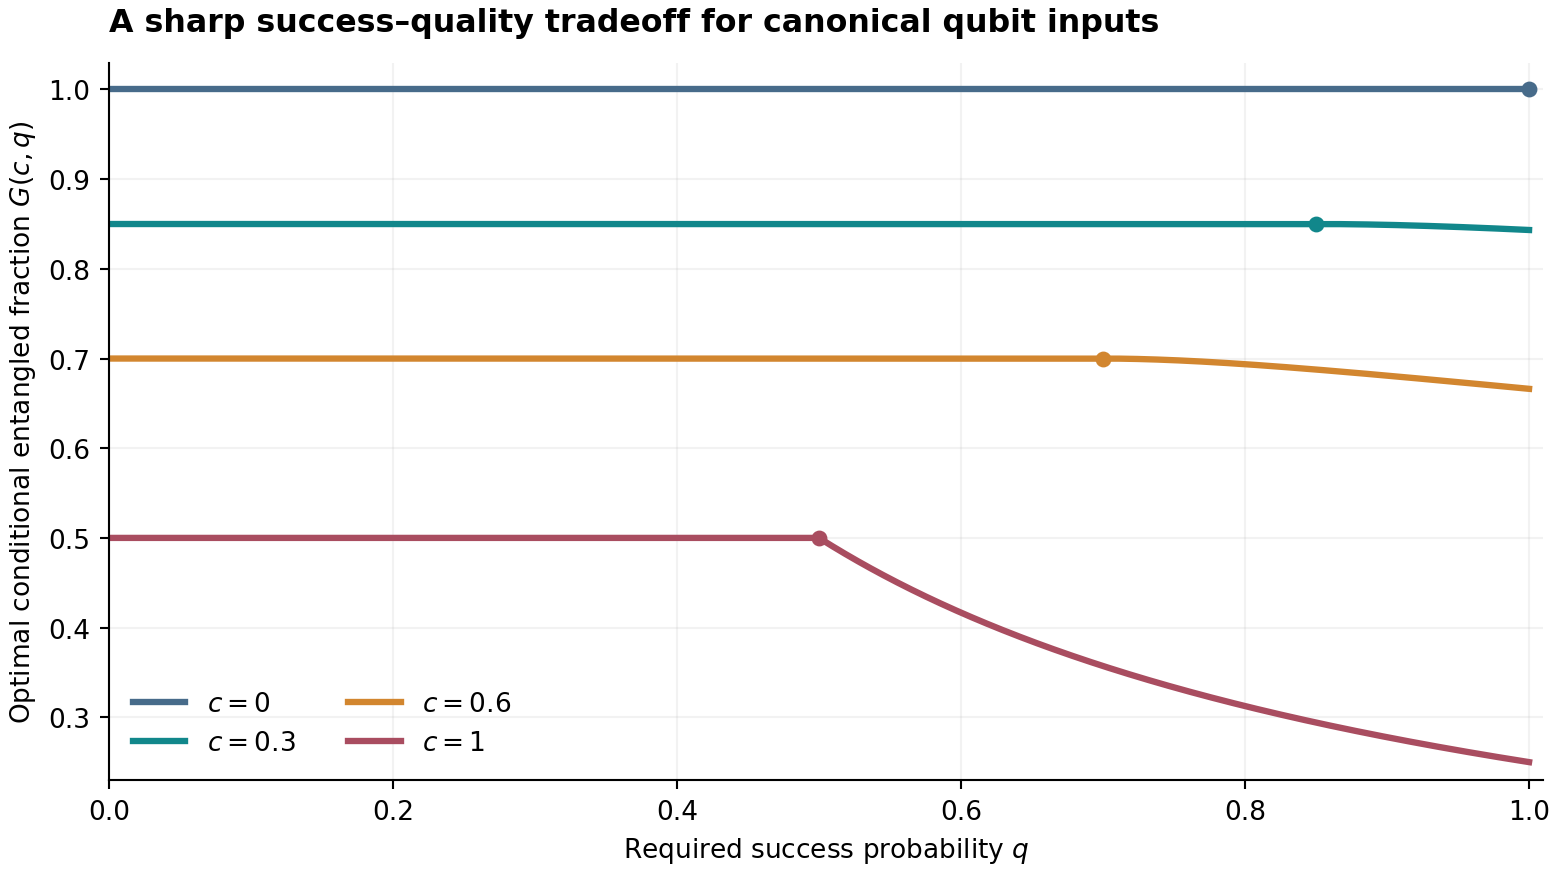
\includegraphics[width=.95\textwidth]{filter_success_frontier.png}
\caption{Exact required-success frontier. A marker identifies $q=1-c/2$, the largest required success at which Milne's centre-only value can still be attained. The curves apply to optimization over canonical inputs with the stated centre and physically allowed Bob filters.}
\end{figure}

\section{Quantitative rigidity of the extracted Schmidt spectrum}\label{sec:cap-stability}
Let $\alpha,\beta,p$ be as in the prescribed-Schmidt theorem, with $p_i>0$, $m_i=\min(\alpha_i,\beta_i)$ and $S=\sum_i\sqrt{p_i m_i}>0$. Let $t=\bra x\tau\ket x>0$ and $w=\tau x/\sqrt t$, and write $q_i$ for the decreasing squared Schmidt coefficients of $w$. The original proof gives $q_i\le m_i$ and
\[
 \sqrt t\le\sum_i\sqrt{p_i q_i}\le S.
\]
\begin{theorem}[Individual cap-deficit control]\label{thm:cap-stability}
For $\epsilon=S^2-t$,
\[
 \boxed{\sqrt{p_i}\,S\,(m_i-q_i)\le2\sqrt{m_i}\,\epsilon\quad\text{for every }i.}
\]
Consequently, writing $p_{\min}=\min_i p_i$ and $m_{\max}=\max_i m_i$,
\[
 \sum_i(m_i-q_i)
 \le\frac{2\sqrt{m_{\max}}}{S\sqrt{p_{\min}}}\,\epsilon.
\]
The residual positive matrix $\tau-ww^\dagger$ therefore has trace at most $1-\sum_i m_i$ plus this explicit error. At equality every cap is saturated.
\end{theorem}
\begin{proof}
Each nonnegative term satisfies
\[
 \sqrt{p_i}(\sqrt{m_i}-\sqrt{q_i})
 \le S-\sum_j\sqrt{p_jq_j}\le S-\sqrt t.
\]
Multiply by $\sqrt{m_i}+\sqrt{q_i}\le2\sqrt{m_i}$, then by $S$, and use
\[
 S(S-\sqrt t)\le S^2-t=\epsilon.
\]
This proves the individual bound, including $m_i=0$. For the aggregate estimate, first sum the square-root deficits with their weights, rather than summing the individual upper bounds:
\[
 \sqrt{p_{\min}}\sum_i(\sqrt{m_i}-\sqrt{q_i})
 \le S-\sum_i\sqrt{p_iq_i}\le\epsilon/S.
\]
Use $m_i-q_i\le2\sqrt{m_{\max}}(\sqrt{m_i}-\sqrt{q_i})$. This avoids an extraneous factor of $d$. This is spectrum rigidity of the canonical extraction, not a claim of universal trace-distance rigidity to a unique state; the high-dimensional optimizer faces above rule out such a uniqueness claim.
\end{proof}
